\section{Photometry}
\label{sec:photometry}
Photometry, in the context of astronomy, is the technique concerned with measuring the flux of an astronomical object's electromagnetic radiation over large wavelength intervals ($\sim100$nm). This is in contrast to spectroscopy in which the same electromagnetic radiation is split into small wavelength intervals ($\sim1$nm) with a chromatic disperser such as a prism. Nowadays, most of the astronomical photometry is carried out using Charge-Coupled Devices (CCDs) as detectors that count individually the number of photons coming from the celestial sources.

\subsection{Photometric system}
A photometric system is a set of well-defined passbands (or filters) with a known sensitivity to incident radiation. The first known standardized photometric system is the \texttt{UBV} photometric system \citep{Johnson1953}, widely used for star classification, which is composed of three broad bands that cover the ultraviolet (U), blue (B) and visual (V) regions of the spectrum (from $\sim$300~nm to $\sim$650~nm). At present, there are more than 200 photometric systems. One of the most famous is the $ugriz$ system \citep{Fukugita1996} used in the Sloan Digital Sky Survey (SDSS) instrument, whose five bands, shown in gray on Fig.~\ref{fig:sdss_filt}, cover from $\sim$300~nm to $\sim$1000~nm. The three bands $ugr$ are roughly equivalent to the $UBV$ ones, and the remaining three reach into the infrared range, which is very useful to detect and measure light coming from distant galaxies whose spectrum has been substantially redshifted.

Photometric systems can be classified according to the widths of their passbands as: broad band, whose passbands are wider than $\sim30$~nm, such as the \texttt{UBV} or the $ugriz$ systems, and narrow bands, whose passbands are less than $\sim30$nm wide, such as the PAU (subsection~\ref{sec:pau}) or ALHAMBRA~\citep{Moles2008} photometric systems.

\subsection{Flux and Apparent magnitude}
The flux $F$ of an astronomical object is the amount of energy as electromagnetic radiation that we receive from the object per unit area and time. If the electromagnetic radiation passes through a bandpass then the received flux is:
\begin{equation}
F = \int^{\infty}_0 f_\nu(\nu)R_\nu(\nu)d\nu = \int^{\infty}_0 f_\lambda(\lambda)R_\lambda(\lambda)d\lambda,
\label{eq:flux}
\end{equation}
where $\nu$ and $\lambda$ are the frequency and wavelength of the radiation respectively, which satisfy $\lambda \nu = c$, $f_\nu(\nu)$ and $f_\lambda(\lambda)$ are the spectral density fluxes of the object, these are the fluxes per unit frequency and wavelength respectively, and $R_\nu(\nu)$ and $R_\lambda(\lambda)$ are the transmission profiles of the bandpass as a function of frequency and wavelength respectively, which give the probability that a photon with associated frequency $\nu$ or wavelength $\lambda$ passes through the filter.

Fluxes of different astronomical objects, or even of the same object but at different passbands, can differ by several orders of magnitude between them. The logatithmic response of the human eye is well adapted to this wide range of fluxes. In fact, ancient astronomers classified stars according to how many times they seemed to shine with more intensity than other stars. This classification has persisted over time and has been formalized through: 
\begin{equation}
m \equiv -2.5\log{F \over F_0} \Longleftrightarrow F = F_0 10^{-0.4m},
\label{eq:mag}
\end{equation}
where $m$ is called the apparent magnitude of the object and $F$ is the actual flux received from it. The zero subindex indicates that the value of the apparent magnitude is defined with respect to another object with flux $F_0$, which defines the zero point. Different zero points define different magnitude systems, such as, for example, the Vega system in which the star Vega is defined to have an apparent magnitude of zero as measured through all filters (that is, $F_0$ is Vega's flux).

\subsection{The AB magnitude system}
Another widely used system is the AB magnitude system, which is not defined by flux ratios as in (\ref{eq:mag}) but spectral density flux $f_\nu(\nu)$ ratios, in such a way that
\begin{equation}
m^R_{AB} \equiv -2.5\log{ \int^{\infty}_0 f_\nu(\nu)R_\nu(\nu){d\nu \over \nu} \over \int^{\infty}_0 f^\nu_0 R_\nu(\nu) {d\nu \over \nu}} = -2.5\log{ \int^{\infty}_0 f_\lambda(\lambda)R_\lambda (\lambda)  (\lambda / c) d\lambda \over \int^{\infty}_0 f^\lambda_0 (\lambda) R_\lambda (\lambda) (\lambda / c) d\lambda},
\label{eq:magAB}
\end{equation}
where the reference flux is $f^\nu_0=3631Jy$\footnote{$1Jy = 10^{-23}erg \cdot cm^{-2} \cdot s^{-1} \cdot Hz^{-1}$  or $1.51 \cdot 10^7 \cdot photons \cdot m^{-2} \cdot s^{-1} \cdot dlog^{-1}\lambda$ in terms of photons.}~\citep{Oke1983}, which is constant in terms of frequency $\nu$, or $f^\lambda_0 (\lambda) = (c/\lambda^2) f^\nu_0$, which depends on $\lambda$, $c$ being the speed of light. In the second equality we have used the relations $\nu \lambda =c$, $d\nu / \nu = -d\lambda / \lambda$ and $\nu f(\nu) = \lambda f(\lambda)$. In the AB magnitude system a source with constant flux per unit frequency will have the same magnitude value in all bands. If we consider a bandpass infinitely narrow such that $R(\nu) \rightarrow \delta(\nu)$, the previous definition becomes
\begin{equation}
m_{AB}(\nu) = -2.5 \log f(\nu) - 48.6.
\end{equation}

\subsection{Color index}
In the same way that magnitudes quantify how brighter is a celestial object with respect to another, the color index quantifies how bluer or redder it is. It is defined as the difference between the magnitude $m_a$ of the celestial object in one passband $a$ with mean wavelength $\lambda_a$ and the magnitude $m_b$ of the same celestial object in a different passband $b$ with mean wavelength $\lambda_b$ such that $\lambda_a<\lambda_b$. According to the magnitude definition in (\ref{eq:mag}), if $m_a-m_b<0$, the ratio of fluxes between the celestial object $F$ and the object of reference $F_0$ in the two different bands fulfill $(F/F_0)_a>(F/F_0)_b$, so that more flux is coming from the bluer part of the object's spectrum with respect to the reference spectrum and, therefore, the object is bluer than the reference. For example, in the Vega photometric system, the Vega star has $m_V = m_B = 0$, so obviously its color index is $B-V \equiv m_B-m_V = 0$. Therefore, a star with $B-V<0$ is bluer than Vega while a star with $B-V>0$ is redder. 

Color indices are very useful in galaxy surveys to classify galaxies according to their color, which, in a similar way as stars, tell us about its activity, temperature and age. For example, red galaxies, also known as early-type galaxies or ellipticals, are older, with less star-formation activity and with a higher metalicity than bluer ones, which are known as late-type galaxies or starburst galaxies.

\subsection{Absolute magnitude and K-correction}
\label{sec:absolute_mag}
The absolute magnitude $M$ is defined to be the apparent magnitude that a source would have if it were 10 pc away, at rest (i.e., not blue- or red-shifted), and compact. In \citet{Hogg1996} it is shown that its relation with the apparent magnitude is:
\begin{equation}
M = m - \mu - K,
\end{equation}
where $\mu$ is the distance modulus 
\begin{equation}
\mu \equiv 5 \log \left[{D_L \over 10pc} \right],
\end{equation}
where $D_L$ is the luminosity distance, defined in (\ref{eq:DL}), to the source in parsecs, and the last term the $K$-correction 
\begin{equation}
K \equiv -2.5 \log \left[{1 \over 1+z}{\int^{\infty}_{0} f_\lambda \left( \lambda / 1+z \right)R(\lambda)\lambda d\lambda \over f_\lambda(\lambda)R(\lambda)\lambda d\lambda}\right], 
\end{equation}
which corrects for the fact that in an expanding universe the spectrum $f(\lambda)$ of a source at a certain distance is redshifted by $1+z$ (so that $f(\lambda) \rightarrow f(\lambda/1+z)$ according to (\ref{redshift})) and therefore, the passband $R(\lambda$) does not see the same part of the spectrum.

The absolute magnitude is a measure of the celestial object's intrinsic brightness. Note that the distance modulus $\mu = m - M - K$ only depends on the redshift $z$ and the profile of the object's spectrum $f_\lambda(\lambda)$ for a given cosmology $\lbrace \Omega_\omega, H_0 \rbrace$. This is specially useful to constrain cosmology with standard candles such as SNIa (section~\ref{sec:distances}), since their absolute magnitude is known beforehand.

\subsection{Luminosity function}
A quantity closely related to the absolute magnitude $M$ is the Luminosity Function (LF), which is the cumulative distribution of stars or galaxies up to a certain luminosity $L$ (energy per unit time). The Schechter function~\citep{Schechter1976} provides a parametric description of the LF, which in differential form is
\begin{eqnarray}
n(x)dx &=& \phi x^\alpha e^{-x}dx, \\
\mbox{with}\ x &\equiv& {L \over L^*}.
\end{eqnarray}
Since $L \propto F \propto 10^{-0.4M}$ we can write $x$ in terms of the absolute magnitude, $x = 10^{-0.4(M-M^*)}$. The function is parametrized by $\lbrace \phi, \alpha, M^*  \rbrace$, where $\phi$ has units of number density and provides the normalization, $\alpha$ is the power-law slope at high magnitudes and $M^*$ the characteristic absolute magnitude where the power-law profile cuts off.

The galaxy LF may have different parameters for different populations and environments; it is not a universal function. In Figs.~\ref{fig:LF_type} and \ref{fig:LF_redshift} we show examples of LF in the $U$-band calibrated with data from the Hubble Space Telescope (HST) and the Great Observatories Origins Deep Survey (GOODS) \citep{Dahlen2005}. They will be used in chapter~\ref{ch:pau} in order to create galaxy mock catalogs for the PAU survey (subsection \ref{sec:pau}). While in Fig.~\ref{fig:LF_type} galaxies have been grouped in different spectral types such as early-type (Ellipticals), late-type and starburst (spirals and irregulars) galaxies, in Fig.~\ref{fig:LF_redshift} we show the evolution in redshift of the composite (LF) through three different $z$-bins: $0.1<z<0.5$, $0.5<z<0.75$ and $0.75<z<1.0$.
\begin{figure}
\centering
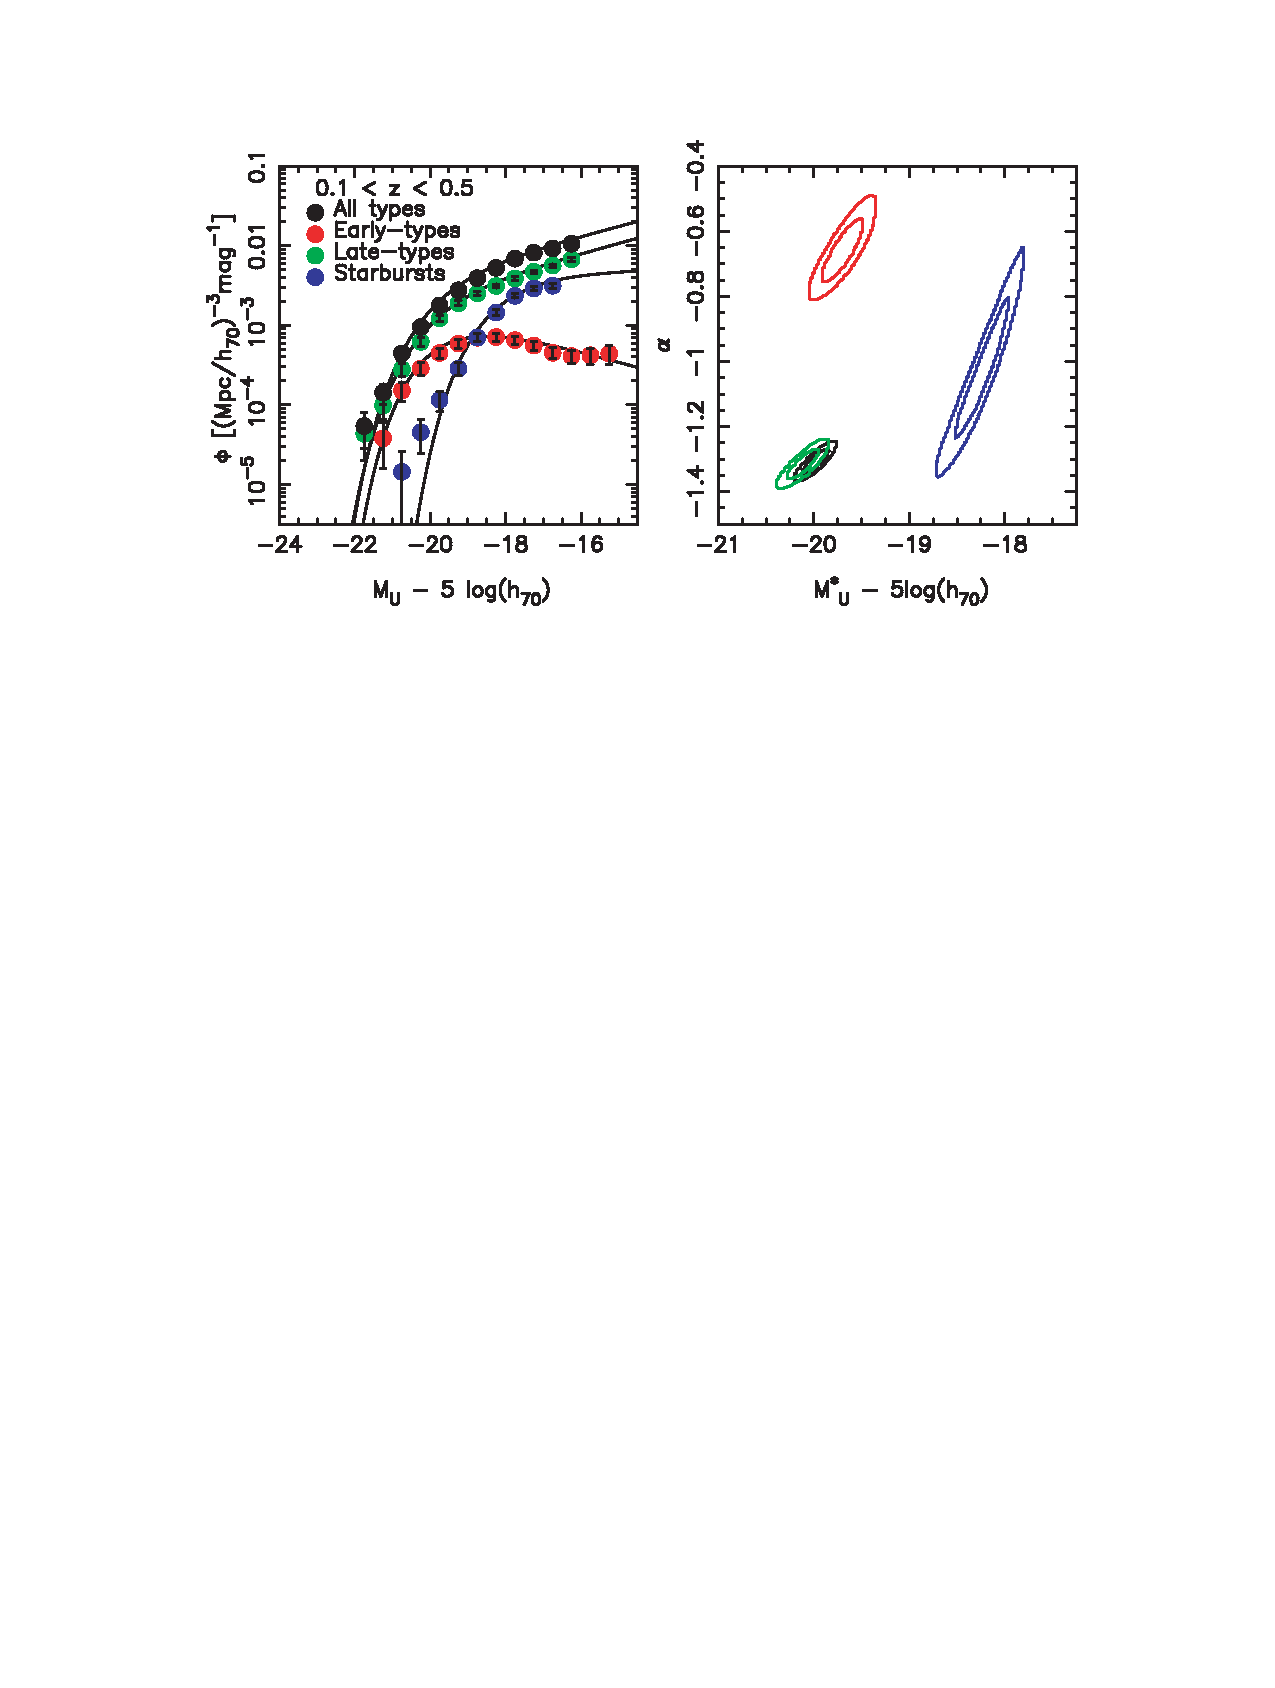
\includegraphics[width=130mm]{./plots/LF_type.pdf}
\caption{Left: Rest-frame U-band luminosity function in the redshift range $0.1<z<0.5$, showing the composite LF (black circles) and the type-specific LFs for early-type (red circles), late-type (green circles), and starburst (blue circles) galaxies. The types are determined from best-fitting spectral templates. Right: The 68.3\% and 95\% error ellipses for $M^*$and $\alpha$ from Schechter function fits to different populations. Figures from \citet{Dahlen2005}.}
\label{fig:LF_type}
\end{figure}

\begin{figure}
\centering
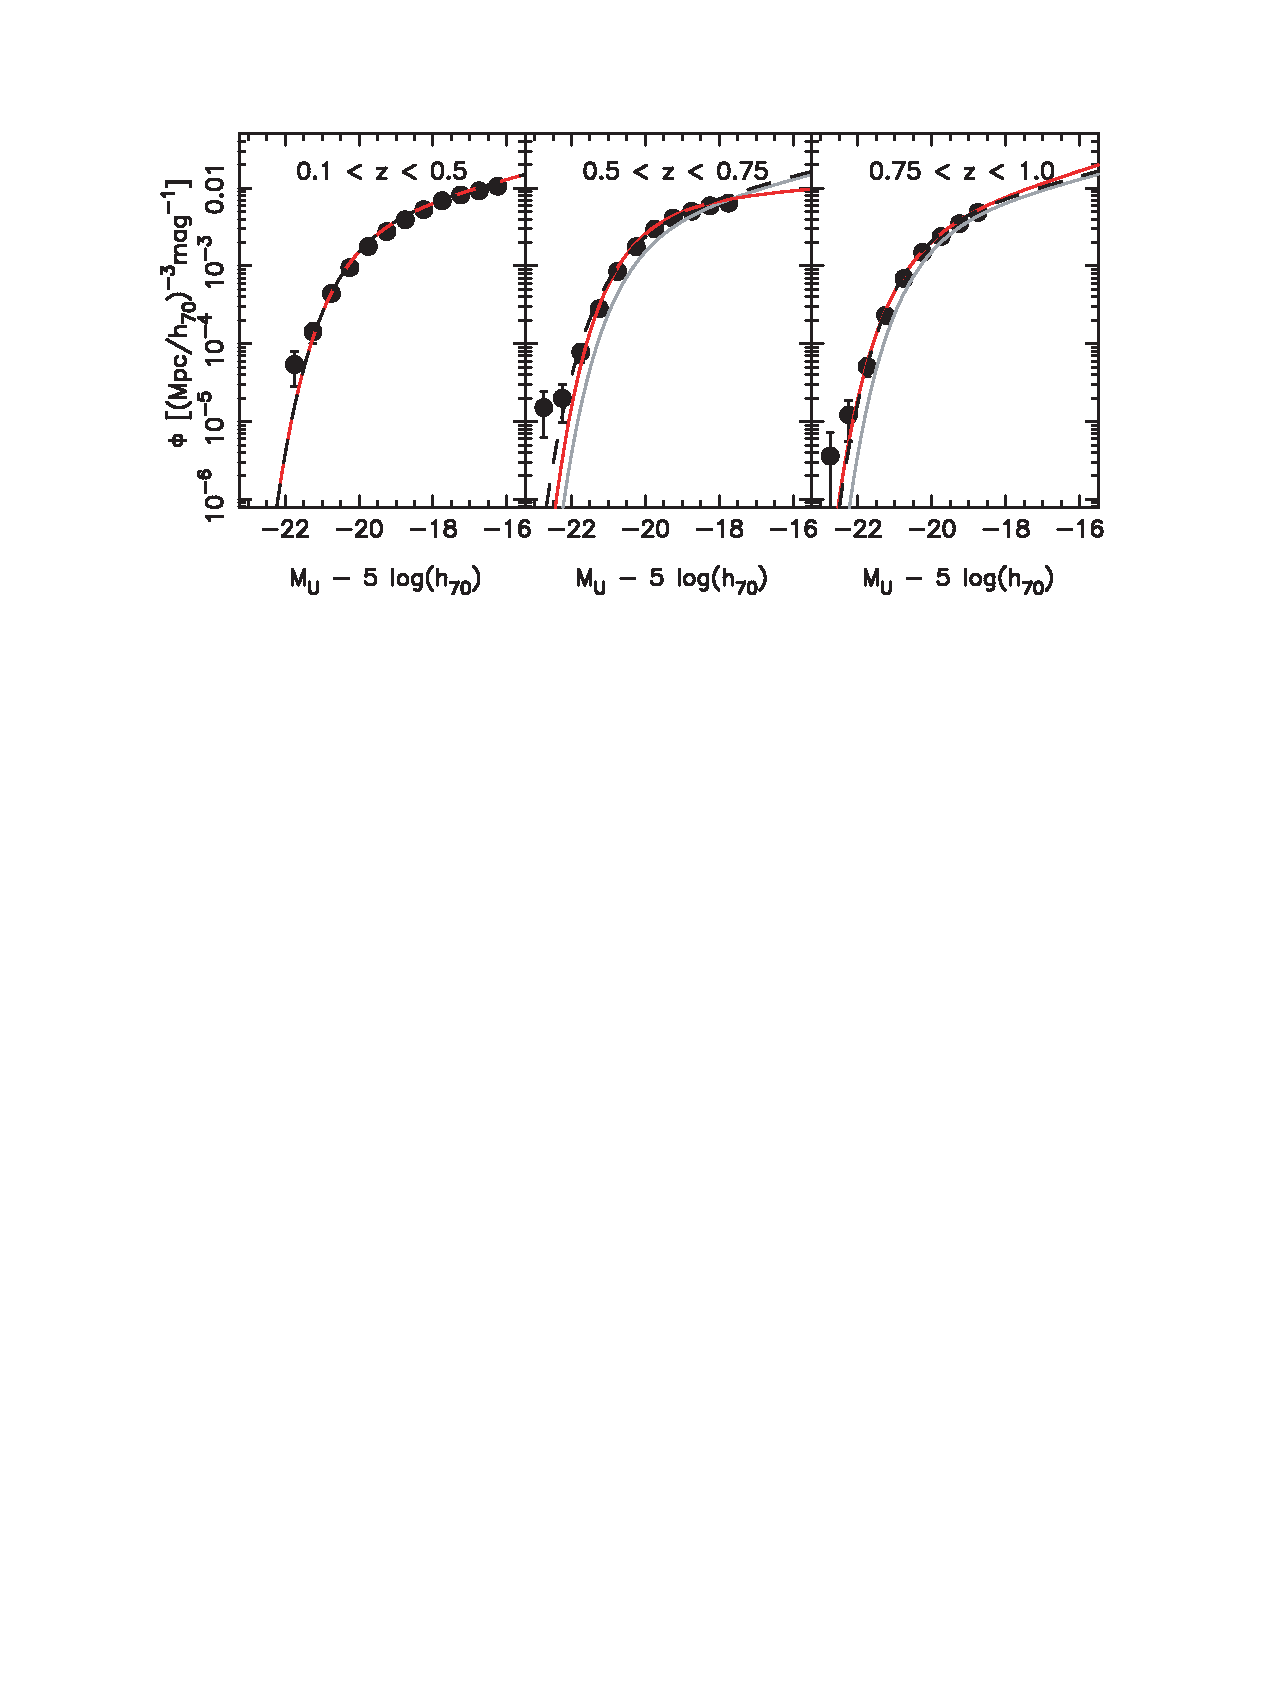
\includegraphics[width=130mm]{./plots/LF_redshift.pdf}
\caption{Rest-frame U-band luminosity function for the redshift intervals $0.1 < z < 0.5$ (left), $0.5 < z < 0.75$ (middle), and $0.75 < z < 1.0$ (right). Solid red lines show the best-fit Schechter function, while dashed black lines show the best-fitting Schechter function for which the faint-end slope, $\alpha$, is fixed to the value measured in the lowest redshift bin. For comparison, we show with a gray line in the mid- and high-redshift bins the best-fitting Schechter function found in the low-redshift bin. Figures from \citet{Dahlen2005}.}
\label{fig:LF_redshift}
\end{figure}
\subsection{Measuring magnitudes}
\label{sec:measuring_mag}
We mentioned that photometry is a technique concerned with measuring the flux of an astronomical object's electromagnetic radiation. In fact, astronomers do not measure fluxes directly, but the number of incident photons $N_{obj}$ that the telescope collects in a certain period of time. These photons are detected and counted by a CCD (Charge-Coupled Device) imaging camera. CCDs were invented in 1969 at AT\&T Bell Labs by Willard Boyle and George E. Smith (Nobel Laureates in Physics in 2009), and rapidly began to be widely used for imaging. A CCD is a two-dimensional matrix of pixels that convert infalling photons into electric charge through the photo-electric effect. Then, by applying weak electrical fields, one can move this charge throughout the pixels until it reaches the edge of the matrix where the cumulated charge is measured and digitalized. In observational astronomy, the Focal Plane (FP) of the telescope where the images of the objects are formed, is covered with several CCDs.  Usually the image of a celestial object covers several pixels, even if it is a point source such as a star or a quasar. The focal plane scale $\alpha$ translates the angular size of a portion of the sky to the number of pixels the image occupies. The integrated flux of the source can be computed directly by summing up the photon counts in a certain region over the FP that encloses the object image, as shown with the green circles in Fig.~\ref{fig:sextractor}. However, often it is difficult to know where the limits of the object are, so on those cases more sophisticated ways are used, such as integrating a model for the 2D-image profile whose parameters are obtained by fitting it previously to the image. 
\begin{figure}
\centering
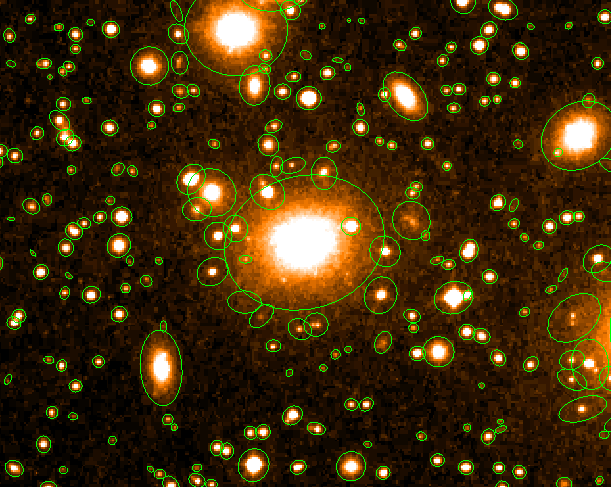
\includegraphics[width=90mm]{./plots/sun226fig.png}
\caption{Illustration of how a software for source extraction, such as the \texttt{SExtractor}~\citep{Bertin1996}, detects galaxies from an image and selects an effective area (green circles) around them where the flux will be integrated.}
\label{fig:sextractor}
\end{figure}
Focusing on the photometry of the SDSS survey (subsection~\ref{sec:sdss}), which will be used in chapter~\ref{ch:odds}, and depending on how they are measured, several magnitudes are defined:
\begin{itemize}

\item \textbf{PSF magnitudes:} For ground based optical telescopes, point source targets, such as stars or quasars, appear on the FP with a certain size due to aberrations introduced by atmospheric turbulence (seeing), diffraction caused by the optics, etc. On those cases, the 2D distribution of light of the image is well described by the Point Spread Function (PSF), which usually would be an Airy pattern from diffraction theory. However, in most cases it can be approximated by a Gaussian profile.

\item \textbf{Model magnitudes:} Just as the PSF magnitudes are optimal measures of the fluxes of stars, the optimal measure of the flux of a galaxy would use a matched galaxy model. Typically, two models are fitted to the 2D image of each object: a pure De Vaucoleurs profile~\citep{vaucouleurs48}
\begin{equation}
I(r)=I_0 e^{-7.67({r/r_e})^{1/4}},
\end{equation}
and a pure exponential profile 
\begin{equation}
I(r)=I_0 e^{-1.68(r/r_e)},
\end{equation}
where $I(r)$ is the brightness at a distance $r$ from the center of the image, $I_0$ is the brightness at the center and $r_e$ an effective radius. The model magnitudes in all the bands will be computed by applying the model (exponential or De Vaucouleurs) of higher likelihood in some reference band filter (the $r$-band in SDSS) and then the same model with the same $r_e$ to the rest of the bands, allowing only the amplitude to vary. This procedure ensures that the color index between different bands is measured through a consistent aperture.

\item \textbf{De Vaucouleurs magnitudes:} The De Vaucouleurs profile is specially good to describe the brightness of elliptical galaxies, therefore the best estimate of the magnitudes for these kind of galaxies is obtained by fitting a pure De Vaucouleurs profile to their image in each band independently. The value of the $r_e$ parameter in some band is called the De Vaucoleurs radius in that band, and is specially useful for galaxy-star separation in catalogs of elliptical galaxies, since they present a $r_e$ value substantially larger than stars. 

\item \textbf{Petrosian}, \textbf{Fiber}, \textbf{Detmodel}, \textbf{Cmodel}, \textbf{Aperture}, \textbf{Auto magnitudes} and many others whose importance is beyond the scope of this work. 

\end{itemize}

Once the counts of photons of the celestial object $N_{obj}$ are estimated, the value of the magnitude is given by Eq.~(\ref{eq:mag}) replacing $F$ by $N_{obj}$ and $F_0$ by the number of counts of the reference object (when observed in the same conditions, i.e. same exposure time). We can also estimate the error of the magnitude as $\sigma_m = |(m \pm \sigma_m) - m| = |- 2.5\log_{10}(F\pm \sigma_F) + 2.5\log_{10}(F)| = |2.5\log_{10}(1 \pm \sigma_F/F)|$, 
where if $F\gg\sigma_F$ then the two solutions are approximately the same. Defining the signal-to-noise (S/N) ratio as the inverse of $\sigma_F/F$, we have that:
\begin{equation}
\sigma_m = 2.5\log_{10}\left(1+{1\over(S/N)}\right).
\end{equation}
The noise, for ground based telescopes, is basically given by adding quadratically three components: the Poisson noise of the signal coming from the object $\sqrt{N_{obj}}$, the Poisson noise of the signal coming from the intrinsic sky brightness $\sqrt{N_{sky}}$ (which is integrated within the same area of the object's image) and the Gaussian noise $RN$ introduced by the electronics in the read-out system. The resulting signal-to-noise ratio expression is:
\begin{equation}
{S \over N} = {N_{obj}\over \sqrt{N_{obj}+N_{sky}+RN^2}}.
\end{equation}

Besides photometric distortions introduced on the measured flux of a celestial object by the Earth's atmosphere (e.g.~the sky brightness and atmospheric absorption) and by the optics of the telescope+camera system, galactic gas and dust between an astronomical object and the observer also absorb and scatter part of the electromagnetic radiation. Since bluer light is more strongly attenuated than redder, dust extinction causes objects to appear redder than expected, a phenomenon referred to as reddening (not to be confused with redshift). In order to measure magnitudes properly, they must be corrected for galactic (Milky way) extinction in each band. In any photometric system, interstellar reddening can be described by a color index excess, defined as the difference between an object's color index and its intrinsic color index (the color index it would have if it was not affected by extinction).
